documentclass[10pt,a4paper]{report}
\usepackage[latin1]{inputenc}
\usepackage{palatino}
\usepackage{lipsum}
\usepackage{pgfplots}
\usepgfplotslibrary{dateplot} 

\begin{document}
\setlength{\parindent}{0ex}

\lipsum[1]\vspace*{2ex}

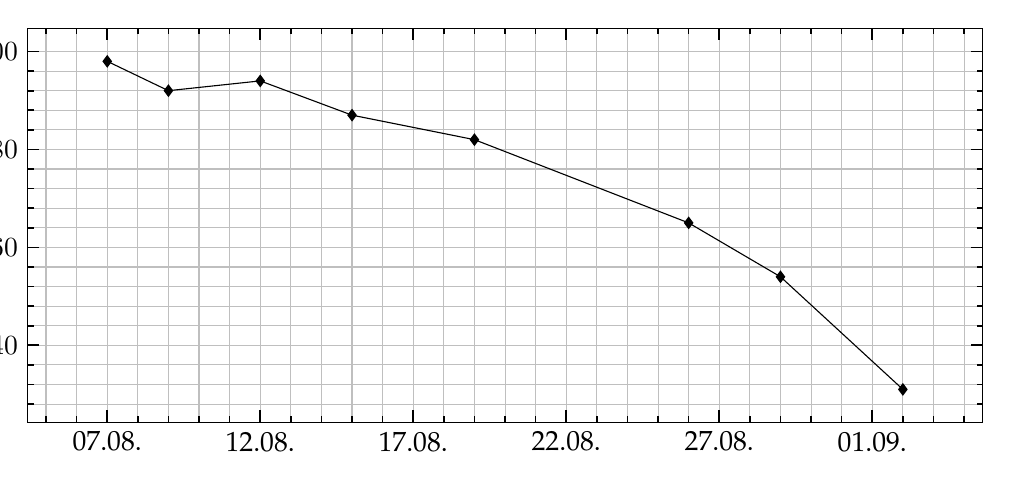
\begin{tikzpicture}[trim axis left]
\begin{axis}[
scale only axis, % The height and width argument only apply to the actual axis
height=5cm,
width=\textwidth,
grid=both,
max space between ticks=40, % To control the number of major ticks
minor x tick num=4,
minor y tick num=4,
major tick length=0.15cm,
minor tick length=0.075cm,
tick style={semithick,color=black}, 
date coordinates in=x,
xticklabel=\day.\month.
]

\addplot[color = black, mark=diamond*] coordinates {
(2009-08-07, 98)
(2009-08-09, 92)
(2009-08-12, 94)
(2009-08-15, 87)
(2009-08-19, 82)
(2009-08-26, 65)
(2009-08-29, 54)
(2009-09-02, 31)
};
\end{axis}
\end{tikzpicture}

\vspace*{2ex}\lipsum[2]

\end{document}
